\chapter{Results}
\label{cha:results}

This chapter offers insight into the outcome of our work. First, the final presentation system is presented, to then cover the results of our early user study. Since one of our objectives was to create a re-usable set of libraries, the usage of the unveil ecosystem from a developer's point of view will also be part of this chapter.

\section{Application}
\label{sec:results-user}
In course of this thesis, we have developed three designated interfaces, one for the listener, one for the speaker and one for the projector. While the projector interface does not have any specific requirements, both the listener and presenter view (see figure \ref{fig:results-user-speaker-presenter}) were optimised for devices with small screens.

Our system offers several ways of interacting with a presentation using ones personal, mobile devices:
\begin{itemize}
\item remote controlling slides,
\item following slides,
\item different paths through presentations,
\item voting and voting creation (on-the-fly),
\item instantaneous reactions and
\item multi-media content sharing.
\end{itemize}
%
With these mechanisms in place, presenters can navigate through slides without the need for proprietary hardware and capture the mood of the crowd through emoji. This is especially useful with increasing audience sizes, as it gets harder to address every participant. The same is true for votings, which can help the speaker to get an idea of the audience' knowledge and interest. When combined with different paths through the application, the progress of a talk or meeting can be controlled by the listeners, tailoring the experience to their needs. Due to our anonymous polling implementation, votings also offer an advantage over hand-raising in smaller audiences. In these settings, the content sharing mechanism shines: by inserting new main and sub-slides, listeners are given full control over the development of a presentation. Related content, notes, questions and comments can all be added by members of the audience, making presentations a collaborative effort. As all these features can be stressful for the speaker, all of them can be enabled or disabled, to their liking.
As the reaction feature of the application has already been covered in detail in chapter \ref{cha:design} and the other mechanisms are fairly self-explanatory, we will now take a detailed look at the voting and content sharing functionality.

\begin{figure}
\centering
\begin{tabular}{ccc}
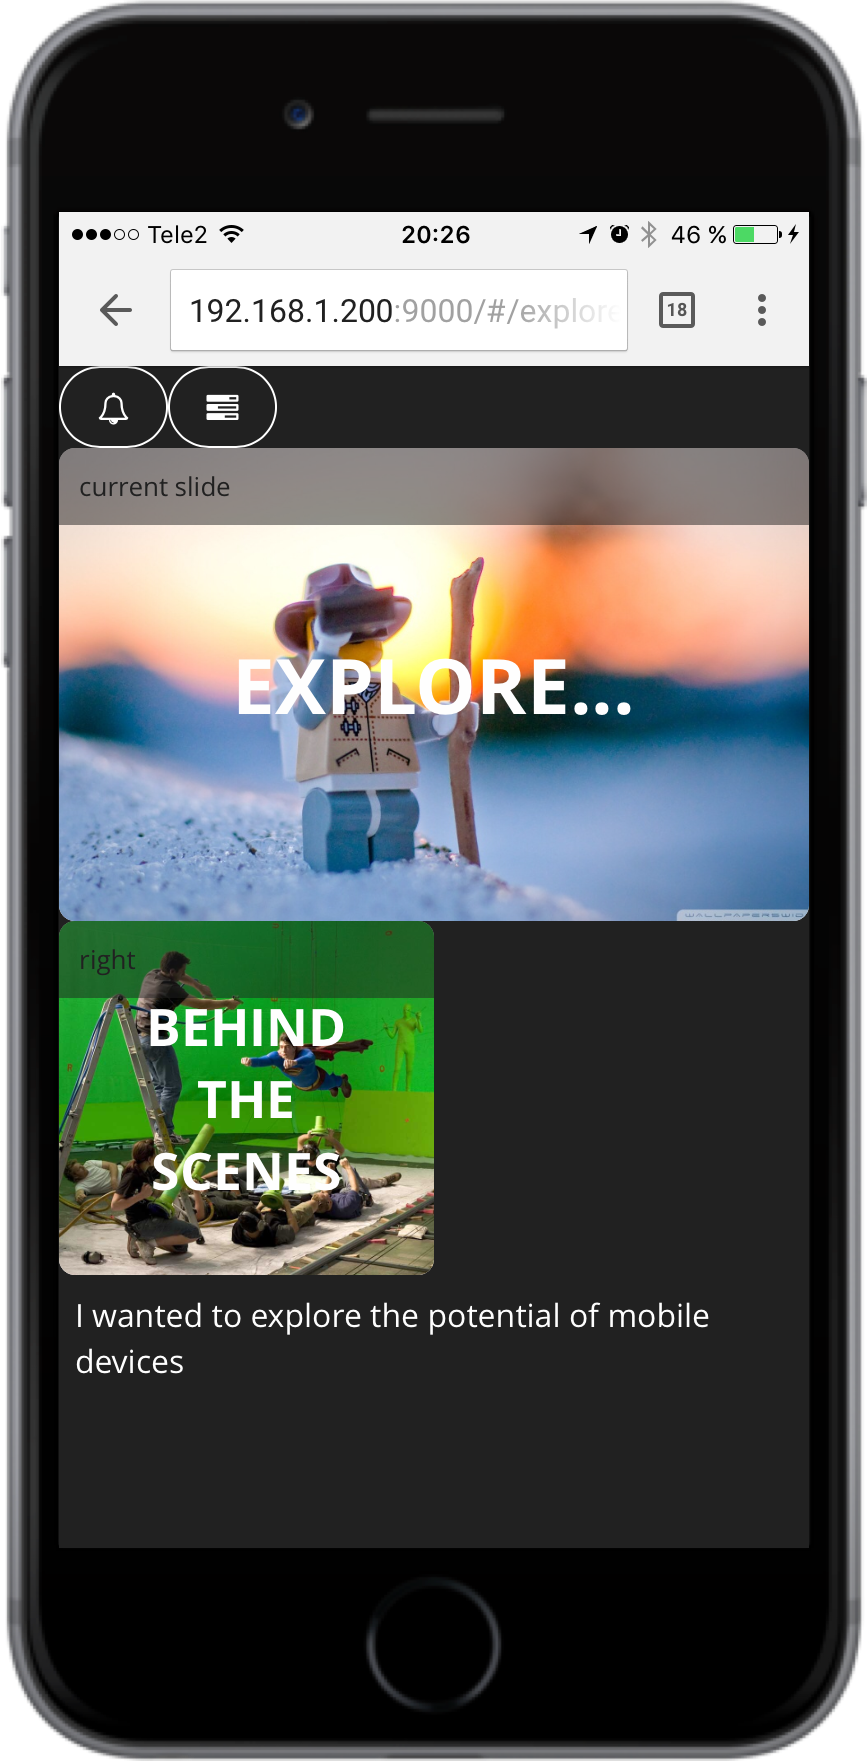
\includegraphics[width=.165\textwidth]{presenter-mode-mobile} &
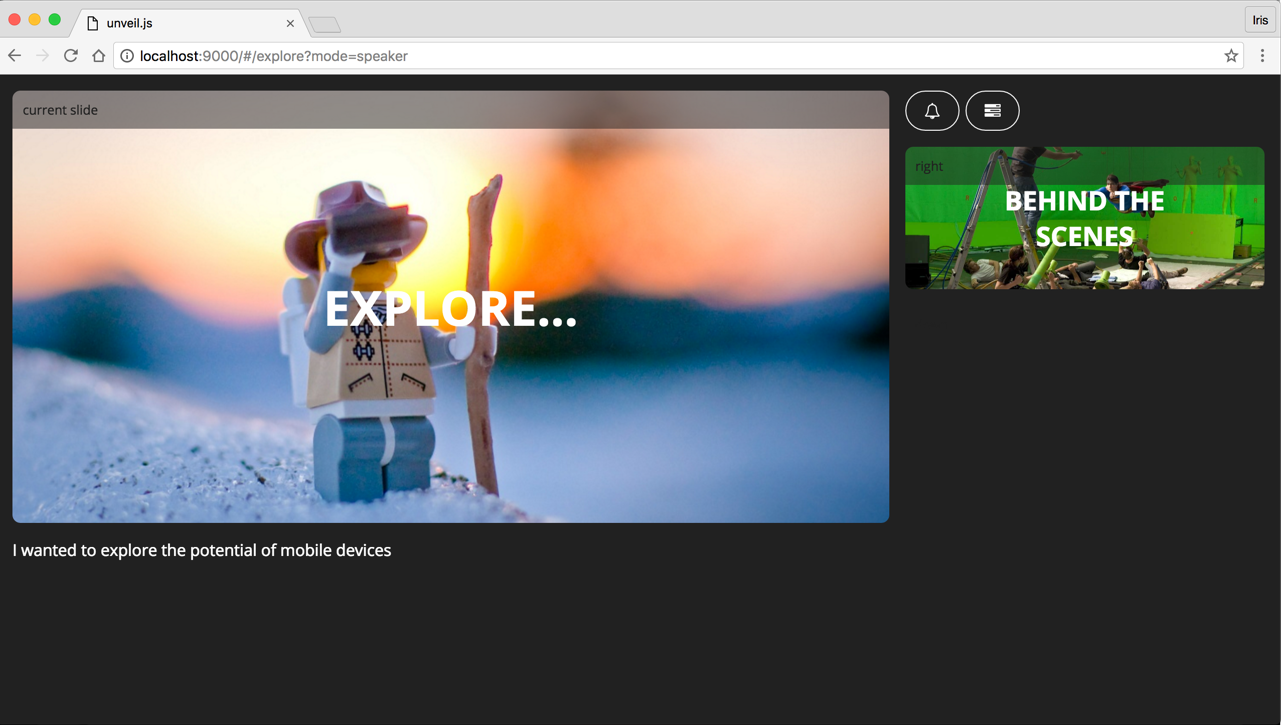
\includegraphics[width=.59\textwidth]{presenter-mode-desktop} \\
(a) & (b)
\end{tabular}
\caption{Speaker Presenter on mobile (a) and desktop (b).}
\label{fig:results-user-speaker-presenter}
\end{figure}

\begin{figure}
\centering
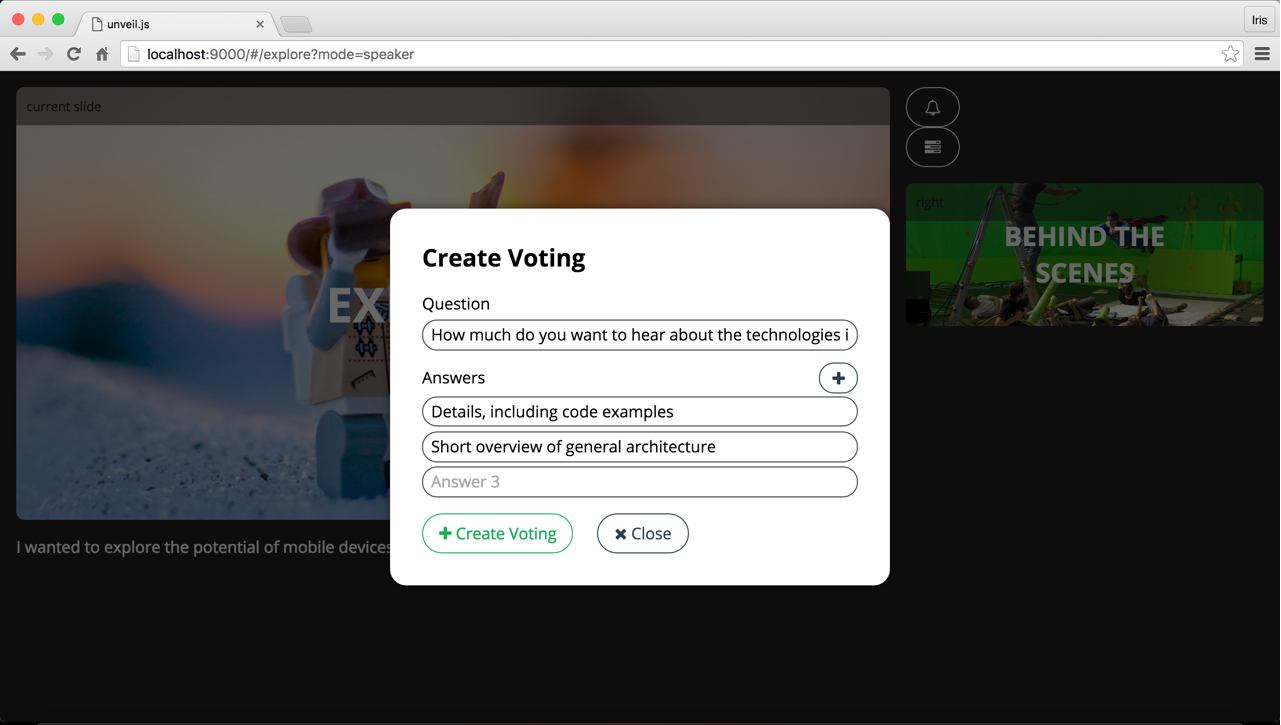
\includegraphics[width=.6\textwidth]{polls-modal}
\caption{Poll creation modal in presenter mode on tablets, laptops and desktops.}
\label{fig:results-user-polls-modal}
\end{figure}

\subsection{Voting}
Votings can be prepared beforehands or on-the-fly -- during the presentation in the speaker interface (see figure \ref{fig:results-user-polls-modal}(a)). After the creation of a poll, the voting starts with the presenter navigating their browser to it.
To ensure as many listeners as possible use their right to vote, all participants are locked to the voting screen for the time of the voting (i.e. until the speaker navigates away from the slide again) and cannot navigate individually anymore. Once a listener votes (see figure \ref{fig:results-user-polls-modal}(b)), they are presented with the current voting results, which are also displayed on the projector. Currently, only single-choice votings are supported by the system, however, free-text or mutliple-choice questionnairs as well as any other kind of form elements could easily be added in the future.

\subsection{Content Sharing}

\begin{figure}
\centering
\begin{tabular}{ccc}
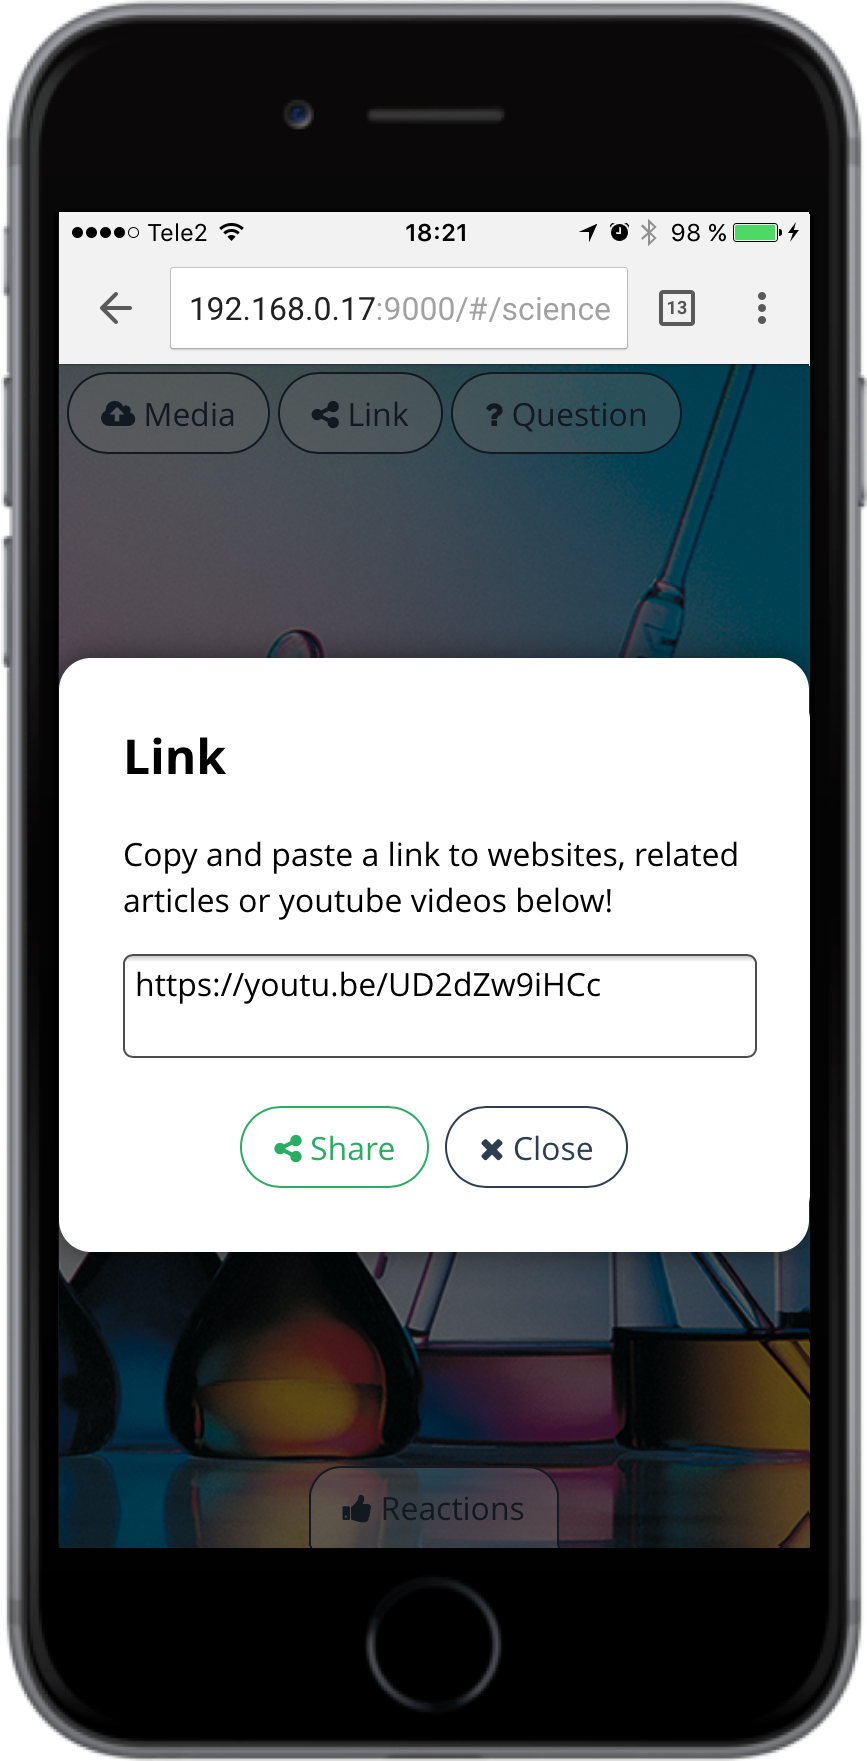
\includegraphics[width=.168\textwidth]{sharing-listener-youtube} &
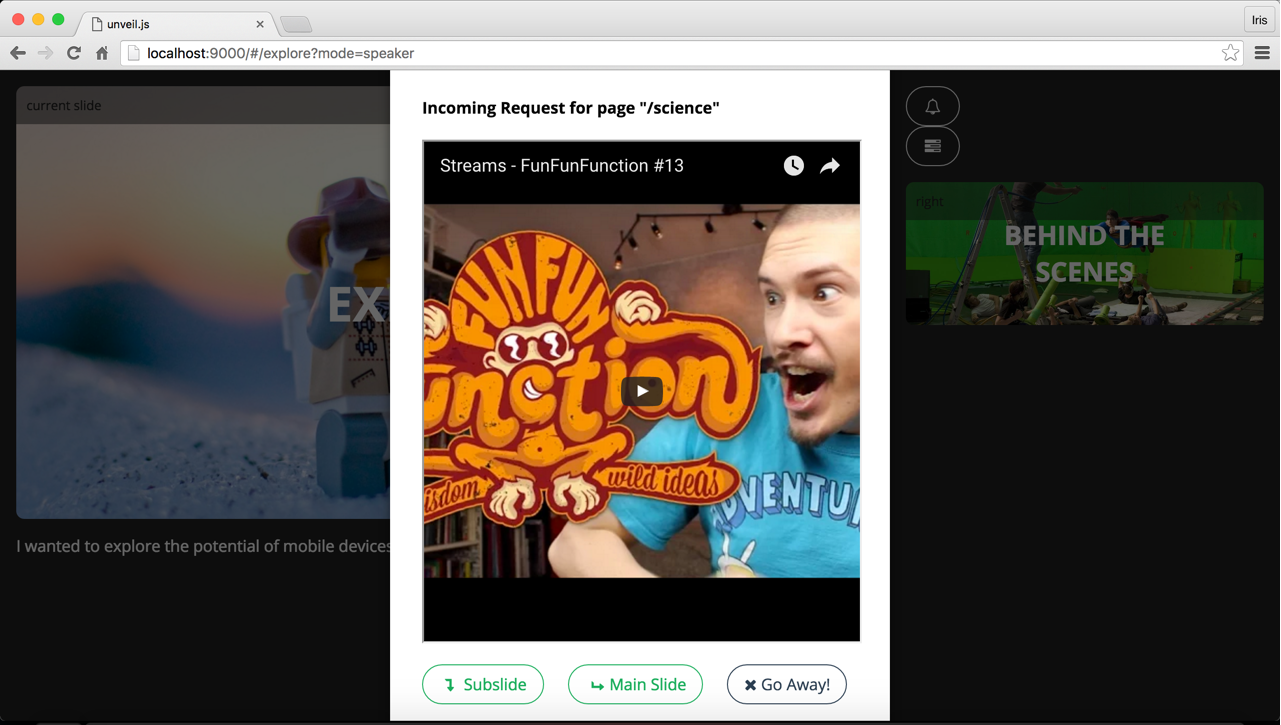
\includegraphics[width=.6\textwidth]{sharing-presenter-youtube} \\
(a) & (b)
\end{tabular}
\caption{Sharing of a youtube video. Request from listener on a phone (a) and accepting-modal in presenter-view on a computer (b).}
\label{fig:results-user-sharing-youtube}
\end{figure}

The seemingly biggest mechanism implemented in course of this thesis is the multi-media sharing feature. Three types of content can be shared in the current implementation:
\begin{itemize}
\item free text (comments and questions),
\item links (to websites, youtube videos or images) and
\item images from the filesystem.
\end{itemize}
The last also includes access to the camera and camera roll on smartphones (see figure \ref{fig:results-user-sharing-picture}) and through that offers a simple interface for uploading hand-written presentation notes, sketches and other related material.

The general process of sharing content is as follows: When a user presses one of the three content sharing buttons in the interface, a modal opens with a text area (free-text and link) or a file-upload (media). After filling in the necessary information, pasting a link or choosing a picture and confirming the action, the presenter instantely receives a content request (see figure \ref{fig:results-user-sharing-youtube}). If the speaker enables the \emph{do not disturb} mode, incoming requests will automatically be added as subslides to the page the request came from. Otherwise a modal will open in the speaker interface, displaying the content and offering to add the content as main slide, subslide or not at all. If the presenter chooses to accept the new content, a new slide will be added with a quote (free text), embedded video or website, or an image.

\begin{figure}
\centering
\begin{tabular}{ccc}
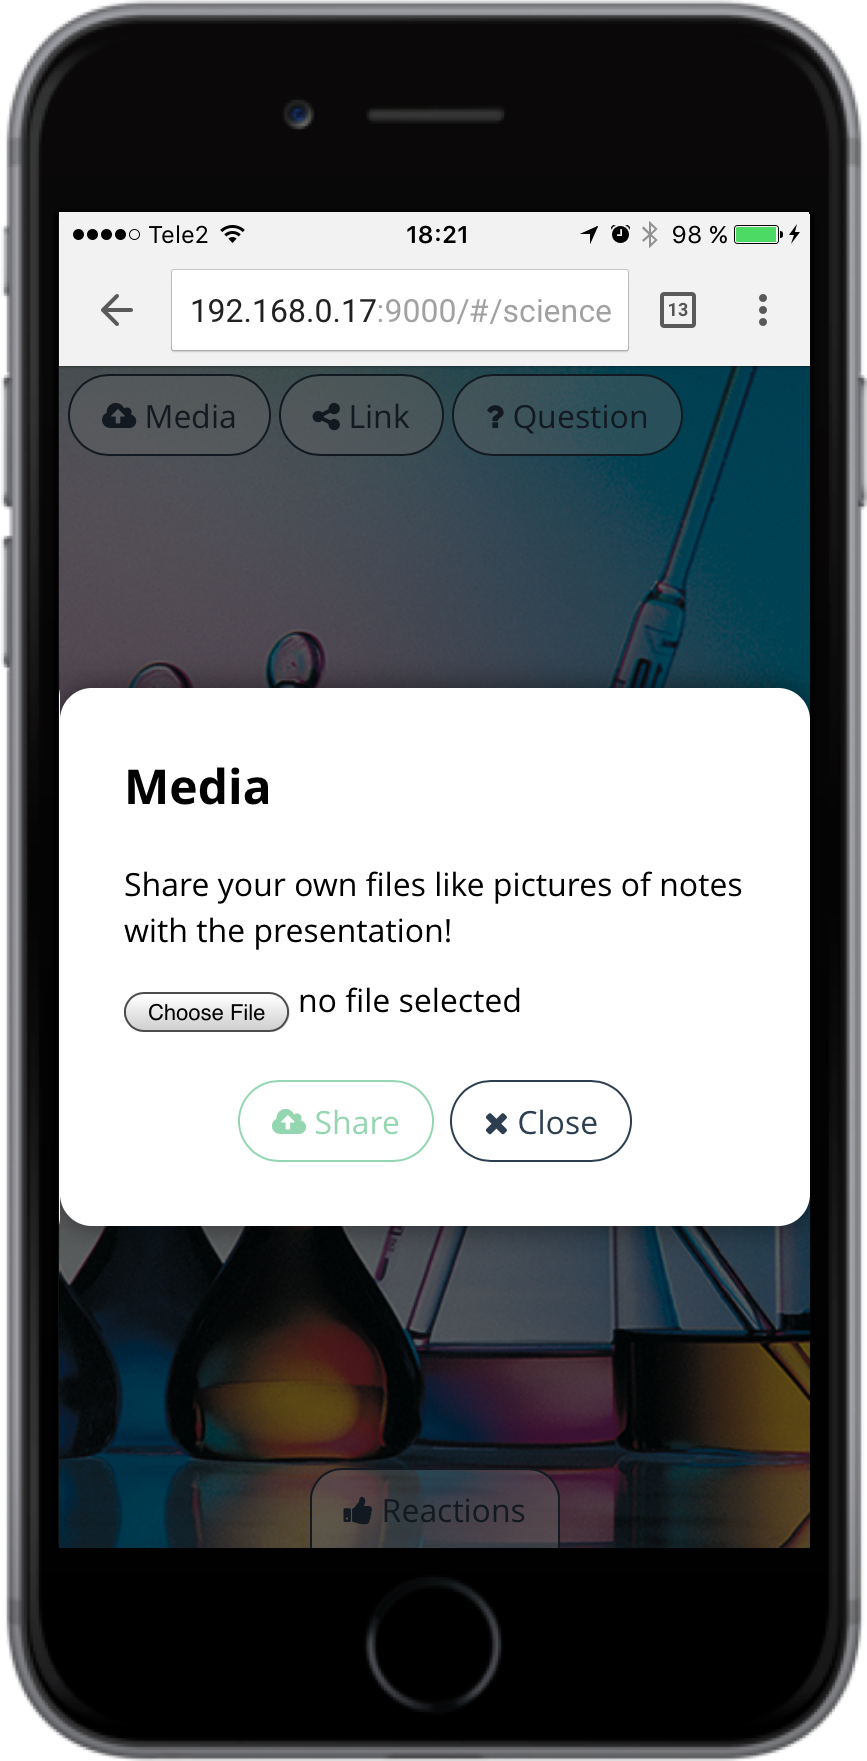
\includegraphics[width=.168\textwidth]{sharing-listener-1} &
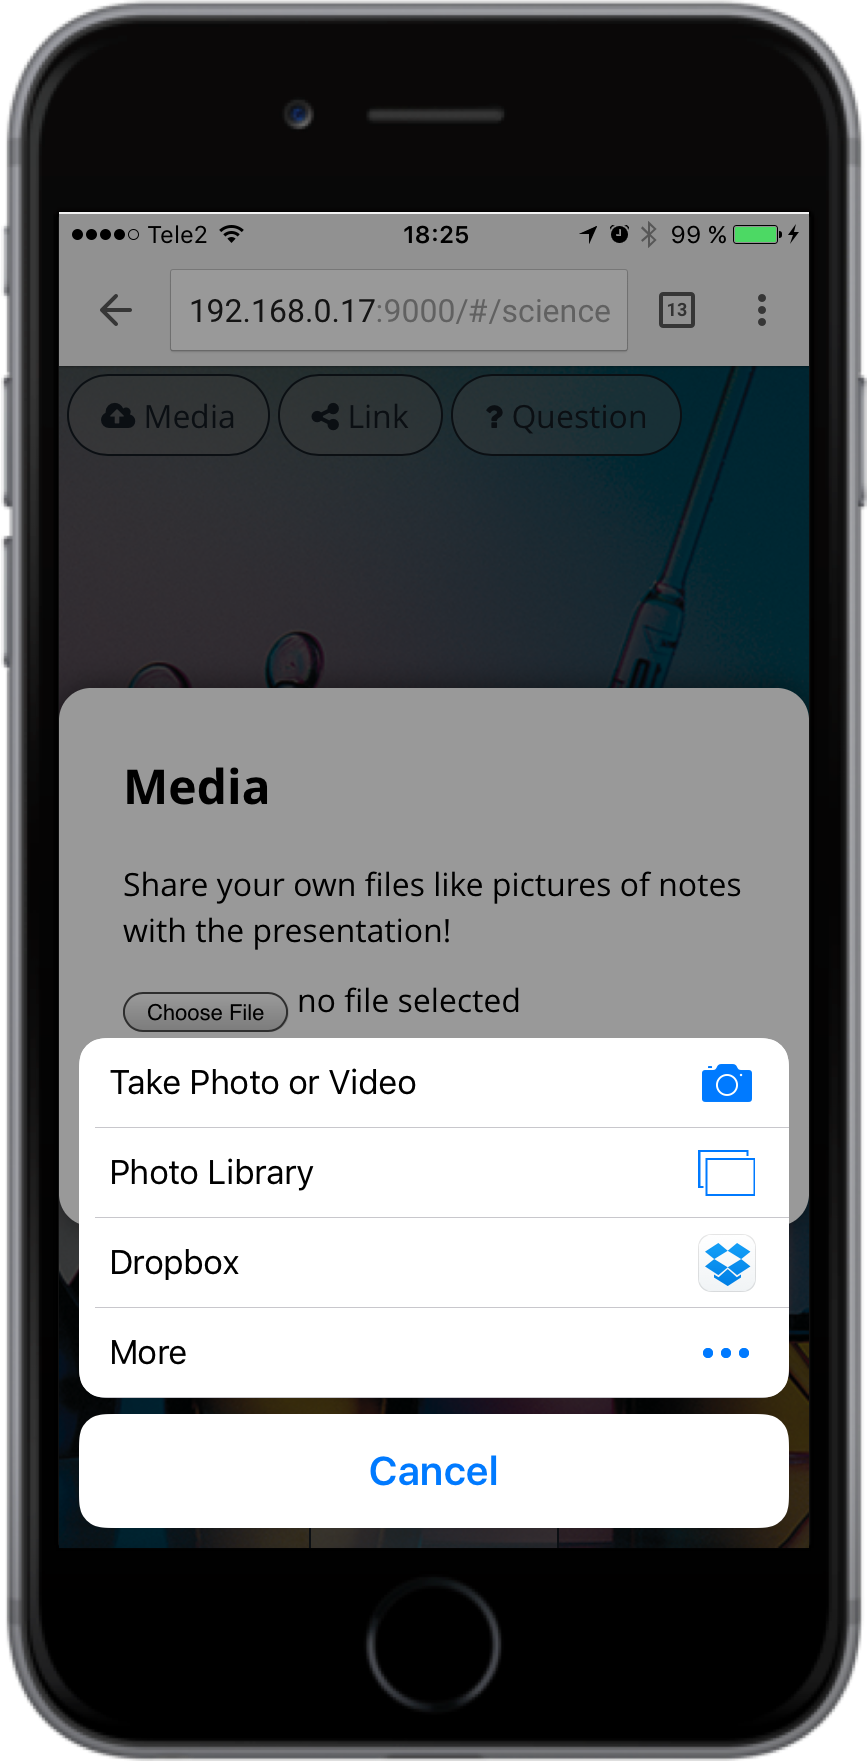
\includegraphics[width=.168\textwidth]{sharing-listener-2} &
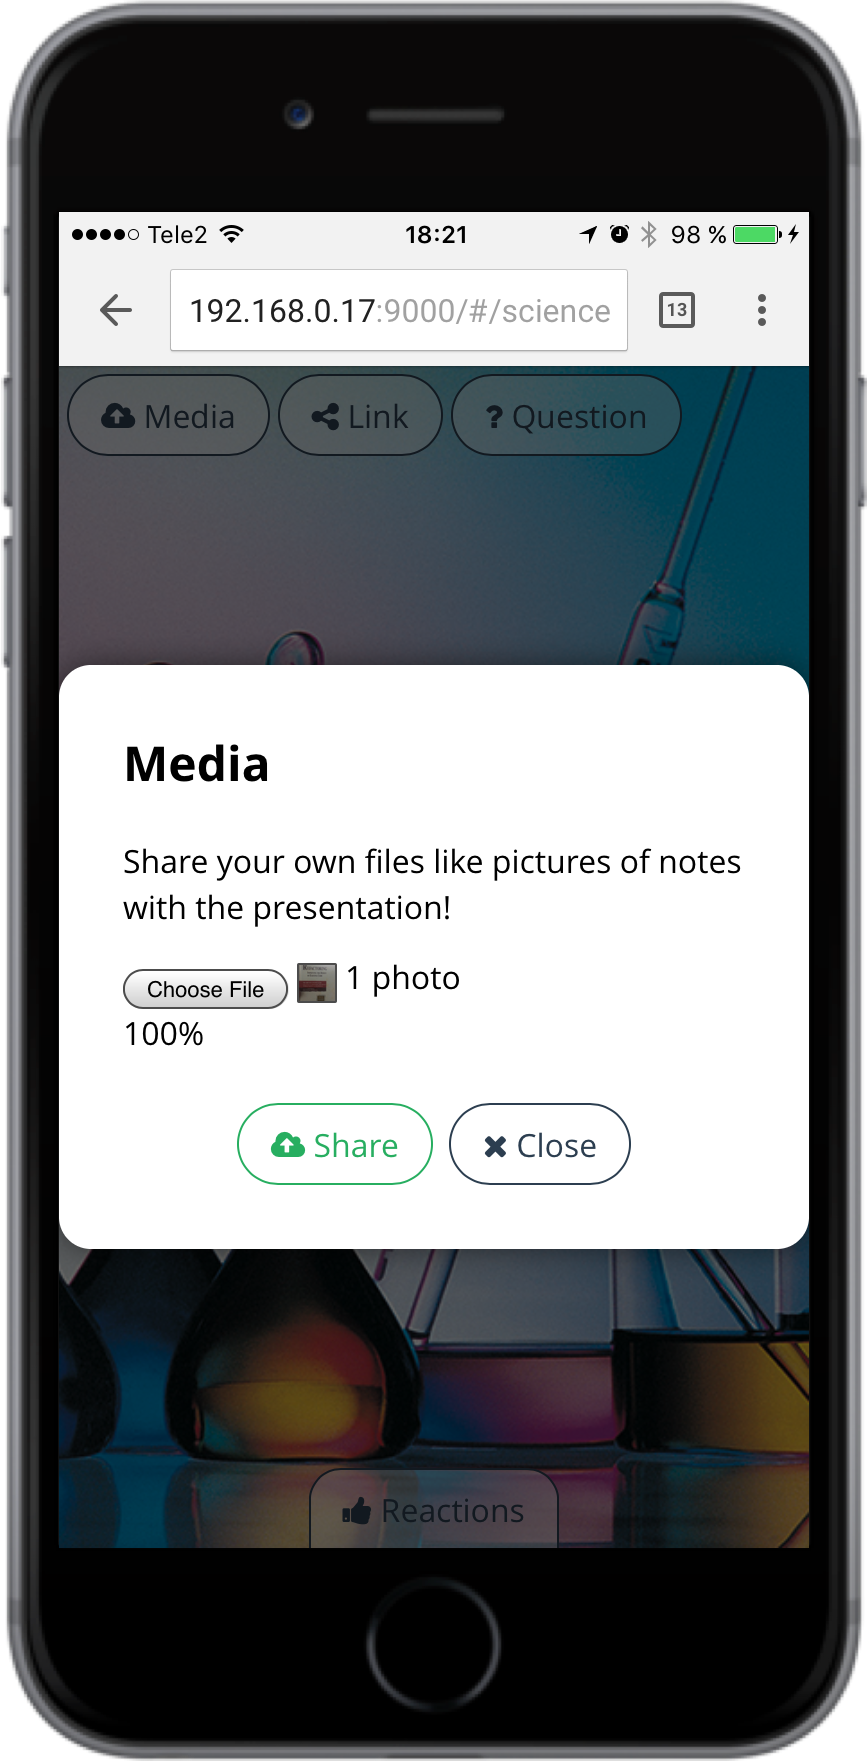
\includegraphics[width=.168\textwidth]{sharing-listener-3} \\
(a) & (b) & (c)
\end{tabular}
\caption{Sharing of a picture from an iPhone's browser (Google Chrome on iOS $9.3.4$) in listener mode. First, the listener opens the \emph{Media} sharing feature (a). Then a file can be chosen from different sources, such as the camera roll, or a new picture can be taken (b). In a last step, the picture is uploaded to the application and can then be shared (c).}
\label{fig:results-user-sharing-picture}
\end{figure}

In our opinion, all these mechanisms combined offer a good starting point for creating more interactive and engaging presentations. The potential of the developed features will be discussed in the next section.

\section{User Study}
\label{sec:results-study}

\begin{figure}
\centering
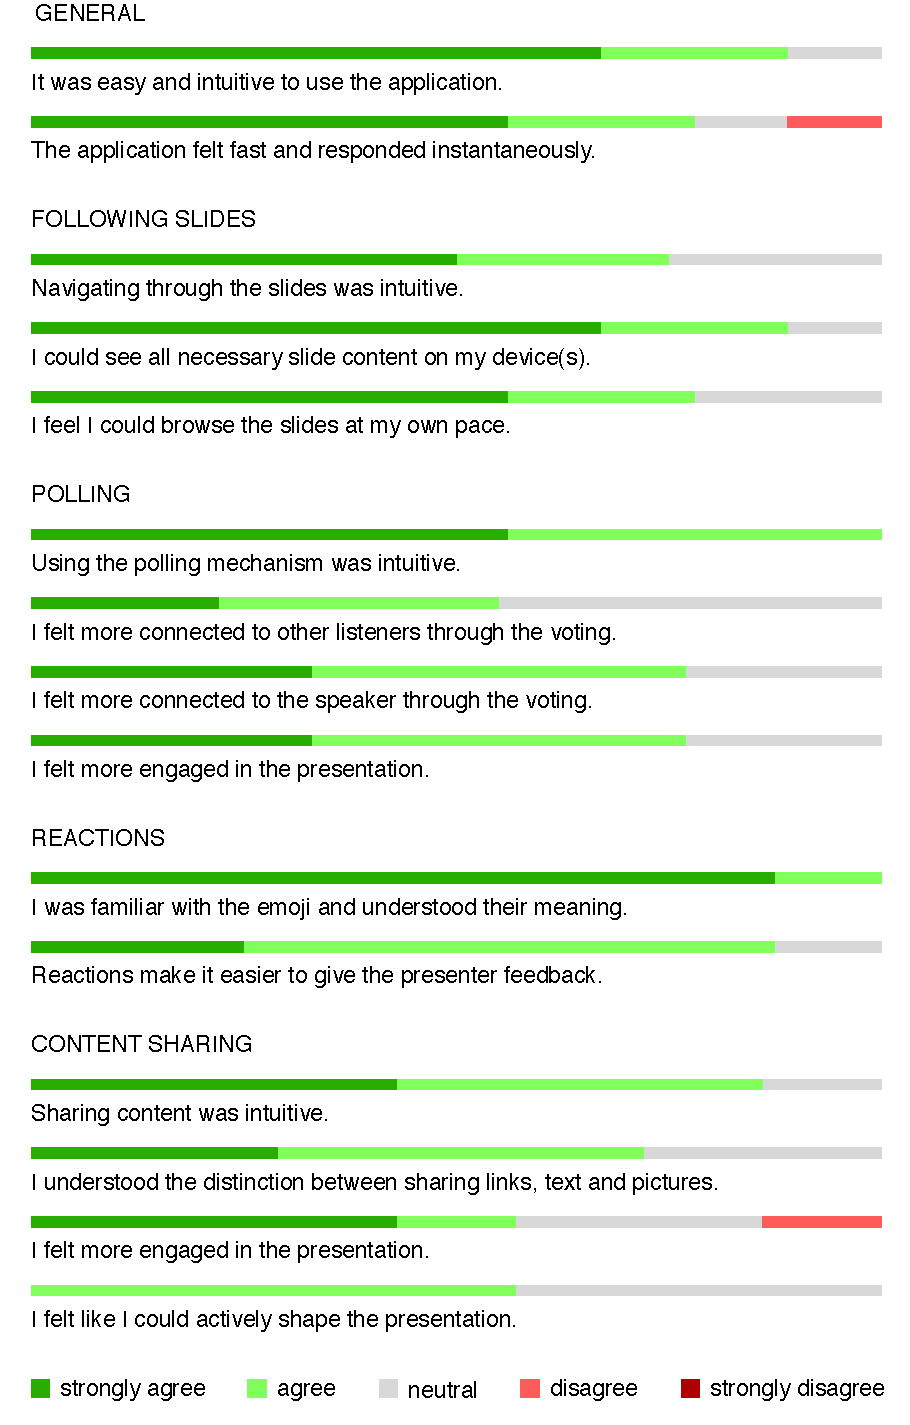
\includegraphics[width=\textwidth]{results}
\caption{User study results, per mechanism. Participants were asked to report their agreement or disagreement to given statements on a 5-point Likert scale.}
\label{fig:results-study-results}
\end{figure}

To measure the result of our work, we deployed the developed system in a presentation at the digital agency Oakwood Creative AB in Stockholm and asked the listeners to fill out a questionnaire (which can be found in the appendices). The results are summarised in figure \ref{fig:results-study-results}, a discussion follows in chapter \ref{cha:discussion}.

The information gathered from the questionnaire consisted of general information about the device(s) the participants used, statements regarding the different mechanisms, which were weighted on a 5-point Likert scale, as well as an area for general feedback for each feature. The given presentation had all interactive mechanisms activated and included a poll about how rude the listeners perceived smartphone use in meetings and presentations. There was, however, only one path through the presentation, so this mechanism was not covered in the user study. The entire questionnaire can be found in the appendices.
In total 9 people, all working in digital marketing, participated in the study. 7 of them used an iPhone to follow the presentation, one used a laptop. One participant interacted with the presentation both on a laptop and an iPhone. Most of the participants chose Safari as their browser on the phone (7 out of 8) and both laptop users chose Chrome.

The vast majority of users agreed or strongly agreed that the application was generally easy and intuitive to use (88.89\%). 77.78\% of the listeners also agreed or strongly agreed that the application felt fast and responded instantaneously. These results confirm the design of the user interface and our choice of technologies.

As far as following the slides on the mobile devices is concerned, the participants came to a similar conclusion: 75\% agreed (or strongly agreed) following the slides was intuitive, moreover 88.89\% reported they were able to see all necessary slide content on their devices. Furthermore, 77.78\% of the participants agreed or strongly agreed the mechanism made it possible for them to browse the slides at their own pace, which was the objective of this feature.

The polling feature received the most positive feedback: All users agreed (44.44\%) or strongly agreed (55.56\%) that the mechanism was intuitive to use, moreover participants reported feeling more connected to other listeners (55.55\%) and the speaker (77.78\% ). In total, almost 80\% of the listeners felt more engaged in the presentation through this mechanism (77.78\%), which confirms our approach.

The user acceptance of the instant reaction feature was also overwhelmingly positive: 87.5\% of the listeners (strongly) agreed the mechanism made it easier to give the presenter feedback. Moreover, we were initally concerned about the users' understanding of the emoji used. With 12.5\% of the participants agreeing and 87.5\% strongly agreeing they were familiar with the emoji and understood their meaning, this worry did not prove true.

Somewhat surprising results, however, were recorded with the content sharing feature. While 71.43\% understood the distinction between sharing links, text and images, only 57.14\% said they felt more engaged in the presentation and like they could actively shape the presentation, with 28.57\% respectively 42.86\% feeling indifferent. 85.71\% however, thought the mechanism was intuitive to use, which shows at least the user interface was well designed.

\section{From a Developer's Perspective}
\label{sec:results-developer}

Since one of our declared goals was the creation of reusable, extensible presentation libraries, a few words should also be spent on the usage of the system by other developers. This chapter will therefore go into details of how to set up an unveil presentation (section \ref{sec:usage-setup}), use the components (section \ref{sec:usage-components}) and lastly ways of customising, overwriting and extending behaviour (section \ref{sec:usage-customisation}). The code-examples of this chapter are based on the unveil-client-server repository \cite{unveil-client-server}.

\subsection{Setup}
\label{sec:usage-setup}
% how is everything defined? what has to be included?
% what are the steps of building an application with unveil?
% how are the slides defined? how are they styled? what about the modes?

Since the entire created code is available on npm, the first step in setting up an unveil presentation is to require the necessary libraries \texttt{unveil}, \texttt{unveil-network-sync} and \texttt{unveil-interactive}. In the entry point of the presentation (usually \texttt{index.html}), all bundled JavaScript and CSS-files are included and an HTML document is created which offers a tag that can be used to render the presentation (e.g. a \texttt{div} with the class \texttt{unveil}). For lower the page loading time \cite{yahoo-speeding-up-website}, script tags should generally placed in the \texttt{body} tag, usually before closing said tag.
As soon as this initial page is set up, the actual presentation can be built in an JavaScript file which should also be included here.
In this file, we will call it \texttt{index.js} from now on, all necessary libraries and components are imported:  \texttt{React}, \texttt{ReactDom}, as well as all unveil components that should be used. If any libraries which rely on the communication with the WebSocket server should be used in the presentation, the \texttt{SocketIO} singelton also has to be configured with the address of the server:
\begin{GenericCode}
import { createSocket } from 'unveil-network-sync'
createSocket('http://192.168.0.17:9000')
\end{GenericCode}

\subsection{Building a Presentation}
\label{sec:usage-components}

Once all libraries are imported, the actual presentation can be created. The most important component in this context is \texttt{UnveilApp}, which is imported from \texttt{unveil}. This component holds all the \texttt{Slide}s and is responsible for the configuration of the application (see section \ref{sec:usage-customisation}). Inside the \texttt{Slide} components, all content of the slide and the \texttt{Notes} are placed. Each of the slides will be rendered as common HTML and can include any number of other HTML tags and custom React components (see programm \ref{prog:usage-presentation-creation}). Although strictly-speaking not necessary, it is recommended to give slides (unique) names, since their name will be the id of the rendered HTML component and makes it possible to style components with CSS (see programm \ref{prog:usage-styling}). Additionally, if provided, unveil uses the name of the current slide as the url, allowing for text-based rather than index-based routes.

Other than that, slides can have a \texttt{left}, \texttt{right}, \texttt{up} and \texttt{down} property to allow for several paths through a presentation: All slides are provided as normal slide-sets, but the \texttt{left} and \texttt{right} attributes of the first and last slide of each path point to the previous and next slide shared by the entire presentation. \texttt{Link}s (available in the \texttt{unveil-interactive} package) can be used to access the first slide of each path. Additionally, the interactive extension also offers the components for preparing votings: \texttt{Voting}, \texttt{Question} and \texttt{Answer} (see programm \ref{prog:usage-voting}). The only necessary property for \texttt{Voting}s is the \texttt{name} attribute, which uniquely identifies the voting, as well as exactly one \texttt{Question}-child and an arbitrary number of \texttt{Answer}s.

\begin{program}
\caption{Example styling unveil slides using Sass. In this particular piece of code, the font family of all slides is set and a background image is added to the slide of name \texttt{start}.}
\label{prog:usage-styling}
\begin{CssCode}
.slide
  font-family: 'Open Sans'
#start
  background-image: url('../img/explore.jpg')
\end{CssCode}
\end{program}

\begin{program}
\caption{Creation of a presentation. Sets up two slides as an example. The DOM will be attached to the element of id \texttt{unveil} in the base HTML document.}
\label{prog:usage-presentation-creation}
\begin{JsCode}
ReactDOM.render((
  <UnveilApp modes={modes}>
    <Slide name="start">
      <h1>Unveil</h1>
      <h2>a meta presentation</h2>
    </Slide>
    <Slide name="intro">
      <img src="./img/problem.png" />
      <Notes>Explain initial situation</Notes>
    </Slide>
    ...
  </UnveilApp>
), document.getElementById('unveil'))
\end{JsCode}
\end{program}


\begin{program}
\caption{Creation of votings in unveil. The necessary components have to be imported from \texttt{unveil-interactive}.}
\label{prog:usage-voting}
\begin{JsCode}
<Voting name="like">
  <Question>Do you like these slides?</Question>
  <Answer value="yes">Yes</Answer>
  <Answer value="no">No</Answer>
</Voting>
\end{JsCode}
\end{program}

\subsection{Customisation and Extension}
\label{sec:usage-customisation}

\begin{program}
\caption{Mode definition for setting up an unveil.js presentation. Default (i.e. listener) and speaker modes are omitted to keep the example short, but generally follow the same pattern as the projector mode.}
\label{fig:usage-modes}
\begin{JsCode}
const modes = {
  default: {...},
  speaker: {...},
  projector: {
    controls : [
      NavigationReceiver, MediaReceiver, ReactionReceiver,
      VotingNavigatableSetter, VotingReceiver
    ],
    presenter: Presenter
  }
};
\end{JsCode}
\end{program}

Thanks to unveil's base architecture, it is possible for speakers to entirely customise the entire presentation logic. The most important step is to define the available modes and the presenter and controls which should be loaded in each of them (see figure \ref{fig:usage-modes}). Additionally to the existing controls in unveil and its current extensions, new (presentation) logic can be added by defining ones own React components and assigning them to modes. To interact with the WebSocket server, \texttt{SocketIO} is available from the network synchronisation layer. Data such as the current router state or slide, and the navigator or state subject are accessible through \texttt{UnveilApp}'s context. For examples of existing controls and presenters, the reader is adviced to refer to the implementation of the components discussed in chapter \ref{cha:implementation} \cite{unveil-fork, unveil-network-sync, unveil-interactive}.

Moreover, the \texttt{Router} and \texttt{Navigator} can also be entirely replaced by providing ones own functionality as \texttt{router} and \texttt{navigator} properties in \texttt{UnveilApp}. They only have to follow the same interface as the default implementations. If any additional configuration should be necessary (such as with setting the address of the WebSocket server or customising emoji), singletons or static methods of the components can be used.
